
We use Catmull-Clark (CC) subdivision as our first example (see
Figure~\ref{fig:cc}). CC subdivision can be defined as the combination
of the primal quadrilateral quadrisection (PQQ) scheme and the
Catmull-Clark geometry rules.

{\scriptsize
\begin{verbatim}
template <class Polyhedron, template <class> Rule>
void PrimalQuadQuadralize(Polyhedron& p, Rule<Polyhedron>& r) { ...}

template <class Polyhedron>
void CCSubdivision(Polyhedron& p) { 
  PrimalQuadQuadralize(p, CatmullClarkRule<Polyhedron>());
}
\end{verbatim}
}

For meshes based on PQQ scheme, the footprints of the range vertices
each corresponds to a topology primitive, i.e. vertex, edge or facet,
in the domain (see Figure. \ref{fig:PQQMap}).  The policy class hence
needs to provide the policy functions in each case.

{ \scriptsize
\begin{verbatim}
template <class P> class CatmullClarkRule 
{
public:
  typedef P                                    Polyhedron;
  typedef typename Polyhedron::Vertex_handle   Vertex_handle;
  typedef typename Polyhedron::Halfedge_handle Halfedge_handle;
  typedef typename Polyhedron::Facet_handle    Facet_handle;

  void face_vertex_rule(Facet_handle domain_f,    Vertex_handle range_v);
  void edge_vertex_rule(Halfedge_handle domain_e, Vertex_handle range_v);
  void vertex_vertex_rule(Vertex_handle domain_v, Vertex_handle range_v);
};
\end{verbatim}
}

Each policy function has two input parameters: the domain primitive
and the range vertex. The footprint, defined as the vertices set of
the 1-distance neighbors of the corresponding domain primitive, is
passed as the handle of the primitive. Empolying the incidental
function of the halfedge data structure, the policy designer works on
the simple view of the \italic{local} mesh corresponding to the
footprint. Following codes demonstrate the facet-vertex case.

{\scriptsize
\begin{verbatim}
void facet_vertex_rule(Facet_handle domain_f, Vertex_handle& range_v) 
{
  typedef typename Polyhedron::Point_3 Point;

  Halfedge_around_facet_circulator hcir = domain_f->facet_begin();
  Halfedge_around_facet_circulator hcir_end = hcir;
  range_v->point() = Point(0,0,0);
  do 
    range_v->point() += hcir->vertex()->point();
  while (++hcir != hcir_end);

  range_v->point() /= circulator_size(hcir);
}
\end{verbatim}
}

% Catmull-Clark subdivision

\begin{figure}[htb]
    \centering{\includegraphics[width=10.0cm]{figs/subdivision}}
    \caption{Catmull-Clark subdivision of a quadrilateral control mesh.}  
    \label{fig:cc}
\end{figure}

Loop subdivision uses similar refinement scheme to PQQ scheme except
that it works on the triangle mesh. Hence the footprints of Loop
scheme are same as the CC scheme but without the facet-vertex case.

{\scriptsize
\begin{verbatim}
PrimalTriangleQuadralize(p, LoopRule<Polyhedron>());

template <class Polyhedron>
void LoopSubdivision(Polyhedron& p) 
{ 
  PrimalTriangleQuadralize(p, LoopRule<Polyhedron>());
}

template <class P> class LoopRule 
{
public:
  typedef ...

  void edge_vertex_rule(Halfedge_handle domain_e, Vertex_handle range_v);
  void vertex_vertex_rule(Vertex_handle domain_v, Vertex_handle range_v);
};
\end{verbatim}
}

Doo-Sabin (DS) subdivision is fundamentally different from the primal
subdivision schemes in the aspect of the footprints. As showed in
Figure \ref{fig:PQQMap}, each range vertex corresponds to a
\italic{corner} in the domain mesh. The footprint of the range vertex
is the facet containing the corner.

\begin{figure}
  \centering
  \includegraphics[width=2.5in]{pfigs/DQQRefMap.eps}
  \caption{The correspondence of the domain footprint and the 
           range vertex of the DQQ schemes.}
  \label{fig:DQQMap}
\end{figure}


{\scriptsize
\begin{verbatim}
DualQuadQuadralize(p, DooSabinRule<Polyhedron>());

template <class Polyhedron>
void DSSubdivision(Polyhedron& p) 
{ 
  DualQuadQuadralize(p, DooSabinRule<Polyhedron>());
}

template <class P> class DooSabinRule 
{
public:
  typedef ...

  void corner_vertex_rule(Halfedge_handle domain_e, Vertex_handle range_v);
};
\end{verbatim}
}

The only policy function for the DS subdivision has the halfedge
pointing to the corner as the domain parameter. A demo of policy
function for the regular facet, i.e. the quadrilateral facet, is
listed in the following codes.

{\scriptsize
\begin{verbatim}
void corner_vertex__rule(Halfedge_handle domain_e, Vertex_handle range_v) 
{
  range_v->point() = Point(0,0,0);

  range_v->point() = domain_e->vertex()->point() * 9 + 
                    (domain_e->next()->vertex()->point() +
                     domain_e->pre()->vertex()->point()) * 3 +
		     domain_e->next()->next()->vertex()->point();
  
  range_v->point() /= 16.0;
}
\end{verbatim}
}

For the complete implementation of the subdivision, readers should
refer to the accompanied source codes of this tutorial.
